\section{Untersuchung von Polarisation}

	\subsection{Allgemeines zu dem Aufbau}
	
		\subsubsection{Versuchsmaterialien}
		
			\begin{figure}[ht]
				\centering
				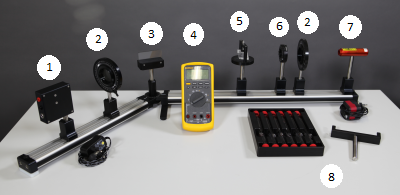
\includegraphics[width=\textwidth]{bilder/s_Materialien.png}
				\caption{Für den Versuch verwendete Materialien.\cite{WWU}}
				\label{fig:Materialien}	
			\end{figure}
			Die für diesen Versuch verwendeten Materialien sind in Abb. \ref{fig:Materialien} dargestellt.
			Bei diesen handelt es sich um
			\begin{enumerate}
				\item eine Photodiode zur Erzeugung von Photostrom durch das einfallende Laserlicht nach der Polarisation
				\item zwei Polarisatoren zum Polarisieren des Laserlichts
				\item eine Glasplatte zur Untersuchung ihres Reflexionsvermögens
				\item ein Messgerät um die Intensität des Lichts dem Photostrom zu entnehmen
				\item ein Kalkspat zur Untersuchung von Polarisation an Kristallen
				\item ein $\lambda/2$-Plättchen zur Drehung der Polarisationsebene
				\item ein Laser zur Erzeugung von Licht, welches polarisiert werden soll
				\item einige Röhren, die mit Zuckerlösungen unterschiedlicher Konzentration befüllt sind, welche zur Untersuchung des Strahlenversatzes in Abhängigkeit der Konzentration dienen.
			\end{enumerate} 
			Für die verschiedenen Teilversuche werden jeweils nur einige dieser Materialien verwendet.		
			Da der Photostrom sehr gering ist, wird die dazu proportionale Spannung, welche ebenso proportional zu der Intensität ist, an der Photodiode gemessen.
			Die Betrachtung der Unsicherheiten, die bei den Materialien auftreten und den Rechnungen auftauchen sind im Anhang \ref{sec:anhang} aufgeführt.
			
		\subsubsection{Polarisation von Licht} \label{sec:Polarisation}
		
			Licht, welches im Wesentlichen eine elektromagnetische Welle mit hoher Frequenz ist, breitet sich als Transversalwelle aus. 
			Das bedeutet, dass der elektrische Feldvektor senkrecht zur Ausbreitungsrichtung schwingt. 
			Polarisation beschreibt die Änderung der Schwingungsrichtung des E-Feldvektors.
			Bei einem Laser tritt das Licht unpolarisiert, bzw. eigentlich in alle Richtungen polarisiert, aus.
			Polarisatoren dienen dazu nur in bestimmte Richtungen polarisiertes Licht durchzulassen.
			Das von ihnen ausgehende Licht wird dann linear polarisiert genannt.
			
			Der Laser und die beiden Polarisatoren werden für alle Teilversuche verwendet.
			
